\documentclass[12pt,fleqn]{article}\usepackage{../../common}
\begin{document}
Ders 1-18

Sonlu Öğeler, 2. Bölüm

Üzerinden geçelim, sistem zayıf form ile işe başlar. Önceki dersin sonunda
Galerkin fikrini tanıştırdık, sürekli diferansiyel denklem yerine onu ayrıksal
temsil etmeye uğraş. Galerkin bunun için bazı deneme fonsiyonları kullanır
onlara $\phi_1,...,\phi_N$ diyelim, ayrıca test fonksiyonları da vardır
(çoğunlukla test fonksiyonları ile deneme, yani $\phi$ ve $v$ fonksiyonları
aynıdır). Bugün işleyeceğimiz bu fonksiyonların nasıl seçildiği ve hazirlik
asamasini gosterdikten sonra bunun verdigi $KU = F$ denklemin nasil
cozuldugu. $K$ nereden geliyor, $F$ nereden geliyor? $F$ bir sekilde alttaki
ikinci denklemin (oktan sonra) sag tarafindan geliyor, $K$ ise sol
tarafindan.. Detaylari simdi gorecegiz.

$$
- \frac{\ud}{\ud x} \left( c(x) \frac{\ud u}{\ud x} \right) = f(x) \to
$$

$$
\int _{0}^{1} c \frac{\ud u}{\ud x} \frac{\ud v}{\ud x} \ud x =
\int _{0}^{1} f(x) v(x) \ud x
\mlabel{1}
$$

ki eger $u(1)=0$ ise $v(1) = 0$ (sinir sarti).

Sonlu ogeler metotunun (FEM) temeli $KU = F$. Ustteki denklemde okun sol tarafi
diferansiyel denklemimiz, sinir sartlari vs ile ``guclu formda'', oktan sonrasi
zayif form, ki onun da kendi sinir sartlari var. Sabit degiskenler guclu formdan
zayif forma geciyor, ama serbest degiskenler gecmiyor. $v$'yi $u$'dan olan ufak
sapmalar olarak gordugum icin eger $u$'yi sabitliyorsam $v$ de sabitleniyor.

Tum bunlari gorduk ama hala ayaklarimiz yere basmadi; bir cok fikirden
bahsettik, ama simdi daha gercek dunyaya baglanacagiz. Gercek dunya demek tabii
$\phi$'lerle alakali, hangi somut fonksiyonlari $\phi$ olarak sececegiz?

Acaba ornek bir $\phi$ ne olabilir? Mesela $x=2$ noktasinda tepe yapan bir
parcali lineer fonksiyon kullanabilirim,

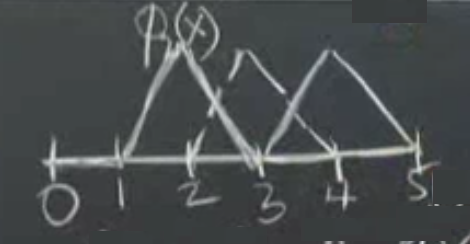
\includegraphics[width=10em]{compscieng_1_18_01.png}

Bu fonksiyona $\phi_2(x)$ diyelim, 1 ila 3 arasinda 2 uzerinde tepe yapiyor
diger yerlerde ya lineer egimi var, ya da degeri sifir. Her $\phi$ maksimum tepe
noktasi 1 olarak secilabilir. Onun sagindaki $\phi_3$ olabilir, benzer bir
fonksiyon sadece 3 degeri bazli tanimli. Buradaki ana amac sistemi basit ogeler
uzerinde insa etmek. FEM'in ana fikri budur; $\phi$ icin basit fonksiyonlar
kullan. Bu basitligin devami olarak $\phi$ ve $v$ fonksiyonlarini ayni sec.

Peki sinir noktalarinda ne olacak? Ustte serbest-sabit problemi cozecegim,
sol uc nokta serbest, sag uc nokta sabit (sinir tanimlanmis). 

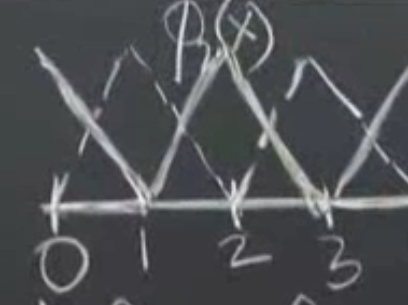
\includegraphics[width=10em]{compscieng_1_18_02.png}

Ustteki resme bakarsak, $x=0$ icin bir ``yarim sapka'' fonksiyonu tanimladim,
$\phi_0$ diyelim, ve eger diger ucgen fonksiyonlara tam sapka dersek bu da yarim
sapka. O noktada $\phi$ ve $v$'lerim kisitli degiller. Boylece elimde bes tane
deneme fonksiyonu oluyor, $\phi_0$, $\phi_1$, $\phi_2$, $\phi_3$, $\phi_4$.

Amac nedir? Yaklasik FEM cozumum $U(x)$'in ustteki basit sapka fonksiyonlarinin
bir kombinasyonu olmasini istiyorum.

$$
U(x) = U_0 \phi_0(x) + ... + U_4 \phi_4(x)
\mlabel{2}
$$

$U_0,..,U_4$ degerleri skalar, tek sayi.. onlar ilk basta bilinmeyen ``agirlik''
degerleri, $\phi$'leri belli sekilde carpacaklar ve bu carpimlarin toplami
yaklasik bir $u$ olacak.

Bu kombinasyonlar neye benzerdi acaba? 

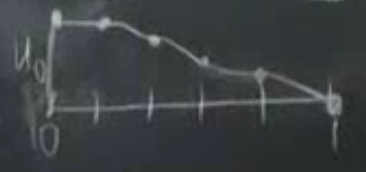
\includegraphics[width=10em]{compscieng_1_18_03.png}

Baslangictaki deger niye $u_0$? Cunku orada tum diger $\phi$ fonksiyonlari sifir
seviyesinde, hemen yandaki $\phi_1$ bile orada sifir ve maksimum $\phi$ deger 1
oldugu icin baslangic degeri $u_0$.

Bu arada Galerkin, ismini tasiyan yontemi bulurken, aklinda erismeye ugrastigi
belli bir cozum fonksiyonu vardi, ve sapka fonksiyonlarini oraya varmak icin
secmisti fakat modern FEM yaklasimlarinda, yazilimlarinda bir temel fonksiyonu
ilk bastan seceriz, problem hakkinda bir sey bilmesek bile. Sapka fonksiyonlari
bu fonksiyonlardan biridir.

Sonlu ogeler temel fonksiyonlari dugum noktalariyla baglantilidir, bu baglamda
sonlu farklilikler (finite differences) metotuna benzer (tabii FD ile esit
aralikla bolmek gerekir, FEM ile bu zorunluluk yok), ogeler dugum noktalarina
oturtuluyor. FEM ile sapka fonksiyonu ozelinde her dugum noktasindaki $u$
degerinin o noktadaki agirlik degeri ile ayni olmasini zorlamis oluyoruz; mesela
1 dugumundeki deger nedir? $u_1$! Cunku orada diger tum sapka fonksiyonlari
sifirdir, sadece $\phi_1$ degeri 1, toplanan tum terimler yokoluyor geriye
sadece $u_1 \phi_1 = u_1$ kaliyor.

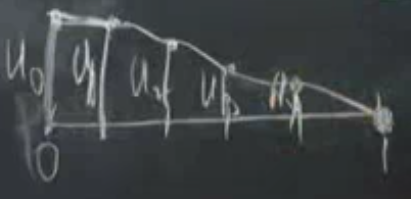
\includegraphics[width=10em]{compscieng_1_18_04.png}

FD benzerligi hakkinda, $KU=F$'i olusturdugumuzda onun bir FD denklemine oldukca
benzedigini gorecegiz, arada yapisal farklar var tabii, FD ile ayriksal
denklemleri biz tanimliyoruz, FEM ile sadece baz ogeleri seciyoruz denklemin
ne oldugunu Galerkin yontemi bize soyluyor.

Simdi bize lazim olan ustteki resimdeki her nokta icin ayri bir denklem, yani
toplam 5 tane denklem. Bu denklemler nereden gelecek? Kritik bir soru.

Bu denklemler zayif formdan gelecekler. Sunu yapiyorum, (1)'deki $u$ yerine
(2)'deki $U$'yu sokuyorum. Ayrica bir $v$ lazim, daha once $v(1)=0$ sarti takip
edilmek suretiyle herhangi bir $v$ olabilir demistik, ama simdi ayriksal forma
gectik, ben de $\phi_i$ fonksiyonlarini $V_i$ fonksiyonlarim icin kullanmaya
karar veriyorum. Boylece,

$$
\int _{0}^{1} c(x) \frac{\ud U}{\ud x} \frac{\ud V_i}{\ud x} \ud x =
\int _{0}^{1} f(x) V_i(x) \ud x
$$

ki $i=0,1,2,3,4$. Boylece 5 tane denklem elde ediyorum, 5 tane $V$ ile ana
formulu ``test ediyorum''. Yani ustteki denklemi 5 tane $V$ icin farkli
sekillerle uretmis oluyorum. Iste 5 x 5 sistemim bu. Neler yaptim simdiye kadar?
Baz fonksiyonlarini sectik, onlari zayif forma sokuyoruz. $\ud U / \ud x$
agirlikli toplamdan geliyor (dikkat tum $V$'leri kullanarak), sonra
$\ud V_i / \ud x$ sokuyoruz, ve entegrali hesapliyoruz. FD durumunda bu
hesap yoktu, entegral hesabi yani, FEM ile var, esitligin hem saginda hem de
solunda.  Esitligin sagindaki entegral her $V_i$ icin bize bir $F_i$ verecek,
yani $F$ vektorunun bir satirini. Tabii $K$ matrisi esitligin solundan
bir sekilde cikacak, nasil birazdan gorecegiz.

Ornek 1

Sag tarafa bakalim once, mesela $i=0$ icin, $f(x)=1$ olsun (ornege gore
boyle) bu durumda $\int_{0}^{1} 1 \cdot V_0(x) \ud x$ entegrali ne
olur? Entegral bir alan hesabidir hatirlarsak, o zaman 

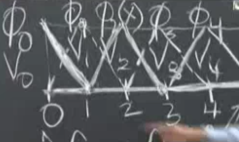
\includegraphics[width=10em]{compscieng_1_18_05.png}

$V_0$ ustteki ilk yarim sapka, o ucgenin alani, eger $x$ ekseni esit araliklarla
bolmussek ve her aralik $\Delta x$ ise,
$(\Delta x \cdot 1) / 2 = \frac{\Delta x}{2}$.

















[devam edecek]


Alttaki Eski Bir Ders Video'sundan Alinmistir

Sonlu Öğeler Metodu (Finite Elements Method)

Bu metot differansiyel, kısmi differansiyel denklemleri (partial differential
equations) yaklaşıksal olarak modelleme ve çözmenin yöntemleridir.

Formül: Başlangıç denklemi

$$ \frac{-d}{\ud x} \bigg( c(x) \ \frac{\ud u}{\ud x} \bigg) = f(x) $$

İki tarafı da  $v(x)$ ile çarpıyoruz ve 0 to 1 sınırlarıyla entegralini alıyoruz.

$$
\int_0^1 \frac{-d}{\ud x} \bigg( c(x) \frac{\ud u}{\ud x} \bigg) v(x)\ud x
= \int_0^1 f(x)v(x) \ud x
$$

Parçalı entegral (integration by parts) formülü şöyledir:

$$ \int y \ud z = y  z - \int z \ud y $$

Ana formülün bölümlerini, parçalı entegrale göre bölüştürürsek:

$$ dz = \frac{-d}{dx} \bigg( c(x) \ \frac{du}{dx} \bigg) dx  $$

$$ z = - c(x) \ \frac{du}{dx}  $$

$$ y = v(x)  $$

$$ dy = \frac{dv}{dx}dx $$

Yukarıda $dz$ içinde $dx$ ve $\frac{1}{dx}$ birbirini iptal eder. Parçalı
entegral formülünün sağ tarafına göre yerlerine koyarsak:

$$
\int_0^1 v(x)\ud x \frac{-d}{\ud x} \bigg( c(x) \frac{\ud u}{\ud x} \bigg)
= - \bigg[ v(x) c(x) \frac{\ud u}{\ud x} \bigg]_{x=0}^{x=1} \int_0^1 c(x) \frac{\ud u}{\ud x} \frac{\ud v}{\ud x} \ud x
$$

Üstteki parçalı entegral açılımında sol taraf entegrale sınır
değerleri aldığında, sağ taraftaki $yz$ sonucunun aynı sınır
değerlerine tabi olduğuna dikkat edelim.

Differansiyel denklemde sınır koşulları $x=1$ durumunda $c(1)u'(1)=0$,
ve $x=0$ durumunda $v(0)=0$ olarak biliniyor. O zaman üstteki
denklemin sol tarafında $x=0$ ve $x=1$ koşulları için tanımlı bölüm $0
- 0 = 0$ olacaktır ve denklemden atılabilir. Geriye kalanlar

$$
\int_0^1 c(x) \frac{\ud u}{\ud x} \frac{\ud v}{\ud x} \ud x
= \int_0^1 f(x)v(x) \ud x
$$

Bu fonksiyonu Galerkin adlı bir matematikçi bulmuş, "zayıf form (weak
form)" olarak adlandırılıyor.

Şimdi diyelim ki n tane test fonksiyonu seçtik $\phi_1(x),..,\phi(n)$
ve bu fonksiyonların $U_j$ sayıları ile çarpımının toplamını, yani bir
tür kombinasyonunu $u(x)$ yerine kullanmaya karar verdik.

$$ U(x) = U_1 \phi_1+ ... + U_n\phi_n $$

O zaman

$$ U'(x) = U_1 \phi_1'+ ... + U_n\phi_n' $$

$$ = \sum_1^n U_j \frac{d\phi_j}{dx} $$

Şimdi $du / dx$ yerine $U'(x)$ koyarsak

$$
\int_0^1 c(x) \bigg( \sum_1^n U_j \frac{\ud\phi_j}{\ud x}\bigg)
\frac{\ud V_i}{\ud x}\ud x
= \int_0^1 f(x)V_i(x)\ud x
$$

Dikkat edelim, $v(x)$ yerine $V_i(x)$ kullandık. Üstteki formül her i için yeni
bir formül "üretecek". Niye $V_i$? Zayıf formdaki $v(x)$ formülünü de zaten biz
uydurmuştuk, yani $v(x)$ biz ne istersek o olur. O zaman bu fonksiyonu n tane
formül üretmek için bir numara olarak kullanıyoruz, n tane formül olunca
matrisin n x n elemanını doldurabileceğiz ve çözüme erişebileceğiz. Ek not,
çoğunlukla $V_i(x)$ için $\phi_i$ sembolü kullanılıyor.

Ayrıca formüldeki $U_j$ kısmını cekip çıkartırsak ve bir vektör içine koyarsak,
geri kalanlar bir $K_{ij}$ matrisi içinde tutulabilir. 

$$ K_{ij} = \int_0^1 c(x) \frac{\ud\phi_j}{\ud x} \frac{\ud V_i}{\ud x} \ud x  $$

Sağ taraf aynı şekilde i tane formül üretir

$$ F_i = \int_0^1 f(x)V_i(x) \ud x $$

Final formül matrix formunda basit bir şekilde temsil edilebilecektir. 

$$ KU = F $$

Örnek

Örnek olarak $-u'' = 1$ denklemini çözelim. Not: Differansiyel
denklemlerde sonuç bulmak demek bir "fonksiyon" bulmak
demektir. Normal cebirsel denklemlerde sonuç bulmak değişkenlerin
"sayısal" değerini bulmak demektir. Birazdan bulacağımız sonuç
$u(x)$ "fonksiyonu" olacak.

Eğer denklem $-u''=1$ ise o zaman bu formülü ana forma uygun hale
getirmek için $c(x) = 1$ olarak almamız gerekir. $-u''=1$ denkleminde
eşitliğin sağ tarafı 1 olduğuna göre $f(x) = 1$ demektir.

Artık $\phi$ fonksiyonlarını seçme zamanı geldi. Bu fonksiyonların
"toplamı" hedeflediğimiz fonksiyonu yaklaşıksal (approximate) olarak
temsil edecek. Örnek olarak seçebileceğimiz bir fonksiyon "şapka
fonksiyonu (hat function)" olarak bilinen üçgen fonksiyonlar
olabilir. Alttaki figürde bu fonksiyonları görüyoruz.

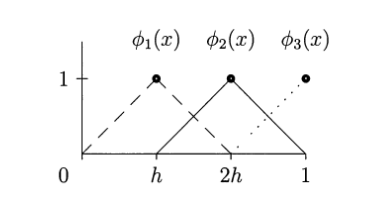
\includegraphics[height=4cm]{fem_hat.png}

Bu figürde x ekseninin h büyüklüğündeki parçalara bölündüğünü görüyoruz. 

Entegralleri hesaplayalım

$$ F_1 = \int_0^1 V_1(x) \ud x $$

Daha önce $V_1$ ve $\phi_1$'i aynı kabul ettiğimizi belirtmiştik. 

Yukarıdaki entegralin aslında bir alan hesabı yaptığını
görüyoruz. Sınırlar $0$ ve $1$ arasında, ama $2h$ ötesinde zaten
$\phi_1$ fonksiyonu yok. $\phi_1$'in alanı nedir? Alan üçgenin alanı:
Taban çarpı yükseklik bölü 2: $2h$, yüksekliği $1$, o zaman alan $(2h
\times 1) / 2 = 1/3$

Benzer mantıkla bakarsak, $F_2$ ile $F_1$ aynı, yani $1/3$. $F_3$ ise
onların yarısı, yani $1/6$.

$K_{ij}$ nasıl hesaplanacak? $c(x) = 1$ olduğu için formülden
çıkarılabilir ve $V_1$ ve $\phi_1$'in aynı olduğuna söyledik:

$$ K_{ij} = \int_0^1 c(x) \frac{\ud\phi_j}{\ud x} \frac{\ud V_i}{\ud x} \ud x $$

$$ K_{11} = \int_0^1 \bigg( \frac{\ud V_1}{\ud x} \bigg) ^2 \ud x  $$

$dV_1/dx$ nedir? Birinci şapka fonksiyonunun türevidir. Bu türeve
bakarsak, $0$ ve $h$ arasında artı eğim (slope) $1/h$, $h$ ve $2h$
arasında eksi eğim $-1/h$ oluyor. Ama kare aldığımız için sonuç aynı,
$1/h^2$. O zaman h = 1/3 olduğuna göre $1/(1/3)^2$, yani $dV_1/dx =
9$.

$$ K_{11} = \int_0^{2/3} 9 \ud x = 9x \bigg|_0^{2/3} = (9)(2/3) - 0 = 6 $$

$K_{22}$ şeklen aynı fonksiyon parçasını temel aldığı için aynı değere
sahip: 6. $K_{33}$ onların yarısı, eşittir 3.

$K_{12}$ farklı eğimlerin çarpımı anlamına gelir, yani $V_1'$ ile
$V_2'$ çarpımı olur. Bu iki fonksiyona bakalım, 0 ile h arasında $V_2$
yok, eğim 0. İkisinin de sıfır olmadığı, çarpımda kullanılabilecek bir
eğiminin olduğu tek aralık h ve 2h arası. Burada $V_1' = -3, V_2 = 3$.

$$
K_{12} = \int_{1/3}^{2/3} (3)(-3) \ud x
= -9x \bigg|_{1/3}^{2/3} = -6 - (-3) = -3
$$

Aynı şekilde $K_{23} = -3$. Ama $K_{13} = 0$ çünkü hiç çakışma yok.

Matrisi doldurursak, 

$$
KU = F
$$

$$ 
\left[\begin{array}{ccc}
    6 & -3 & 0 \\
    -3 & 6 & -3 \\
    0 & -3 & 3     
\end{array}\right]
\left[\begin{array}{c}
    U_1 \\
    U_2 \\
    U_3
\end{array}\right]
=
\left[\begin{array}{c}
    1/3 \\
    1/3 \\
    1/6
\end{array}\right]
$$

Python kodu 

\begin{minted}[fontsize=\footnotesize]{python}
K = [[6., -3., 0],
     [-3., 6., -3.],
     [0., -3., 3.]]

f = [1./3., 1./3., 1./6.]

print np.linalg.solve(K,f)
\end{minted}

\begin{verbatim}
[ 0.27777778  0.44444444  0.5       ]
\end{verbatim}

\begin{minted}[fontsize=\footnotesize]{python}
print 5./18., 4./9., 1./2.
\end{minted}

\begin{verbatim}
0.277777777778 0.444444444444 0.5
\end{verbatim}

Rapor edilen değerler bu denklemin bilinen çözümü $u(x) = x - \frac{1}{2}x^2$ 
ile 0, h, 2h noktalarında (mesh points) birebir uyum gösterdiğini
görüyoruz.  Yani yaklaşıksal olarak differansiyel denklemi çözmeyi 
başardık.

Kaynaklar

[1] Strang, G., {\em Computational Science and Engineering}



\end{document}



